\newpage
\section{Theoretisch Maximum}
\label{sec:eva}

\titlespacing*{\subsubsection}{0pt}{30pt}{10pt}


\subsection*{Deelvraag 1: Wat is het theoretisch maximum aantal kandidaten dat per specifieke bevolkingsgroep gekozen had kan worden in de Tweede Kamer?}

Om het theoretisch maximum te gaan berekenen zullen we als eerst kijken naar de verschillende specifieke bevolkingsgroepen zoals we deze hebben bepaald in de Hoofdstuk \ref{sec:intro}. Deze bevolkingsgroepen zijn: vrouwen, allochtonen, ouderen(met de leeftijd van vijftig jaar en ouder) en provincialen (Nederlanders van buiten de Randstad). 


\paragraph*{Resultaten strategie\"{e}n per bevolkingsgroep.} 
In Tabel \ref{table:S_overzicht} en Figuur \ref{fig:S_overzicht} hieronder zijn per bevolkingsgroep de resultaten van de verschillende strategie\"{e}n te zien. We zien dat strategie 1 voor alle vier de bevolkingsgroepen een hoog rendement zou hebben opgeleverd. Echter zou strategie 4 voor de provincialen het hoogste rendement op hebben geleverd (zie \hyperref[S4P]{strategie 4} van \hyperref[provincialen]{Bevolkingsgroep: Provincialen} in Bijlage \ref{b1}). Strategie 2 zou bij alle vier de bevolkingsgroepen ook een hoog rendement op hebben geleverd. Bij de allochtonen zou het zelfs geen verschil hebben uitgemaakt of strategie 1 of strategie 2 zou zijn uitgevoerd. Het rendement is hetzelfde. Strategie 3.1, strategie 3.2 en strategie 4 zijn op bij de bevolkingsgroep allochtonen niet toegepast vanwege een te klein aantal allochtone kandidaten om uitvoering van deze strategie\"{e}n mogelijk te maken.  

De verschillende strategie\"{e}n worden in dit hoofdstuk in Sectie \ref{vrouwen} toegepast op de bevolkingsgroep vrouwen. Bij deze bevolkingsgroep worden de strategie\"{e}n tot in detail uitgelegd en ondersteund met enkele voorbeelden. Ten behoeve van de leesbaarheid zijn de andere drie bevolkingsgroepen naar Bijlage \ref{b1} verplaatst. Tevens wordt in de bijlage van deze bevolkingsgroepen enkel het resultaat en de analyse getoond. Voor een getailleerde uitleg van uitwerking van de strateg\"{e}n, ga naar Sectie \ref{vrouwen} of ga door naar Hoofdstuk \ref{h5}

\begin{table}[h]
\captionsetup{skip=-2pt}
\begin{center}
\begin{footnotesize}
\begin{tabular}{lrrrrr}
\toprule
{} &  Strategie 1 &  Strategie 2 &  Strategie 3.1 &  Strategie 3.2 &  Strategie 4 \\
\midrule
Vrouwen      &         \hyperref[S1V]{121} &          116 &             91 &            101 &          121 \\
Allochtonen  &           34 &           34 &            n.v.t. &           n.v.t. &          n.v.t. \\
Ouderen      &           89 &           84 &             77 &             69 &           89 \\
Provincialen &          138 &          131 &            103 &            120 &          142 \\
\bottomrule
			
			
\end{tabular}
\end{footnotesize}
\end{center}
\caption{Overzicht van de resultaten per bevolkingsgroep in aantal zetels per strategie.}
\label{table:S_overzicht} 
\end{table}


\begin{figure}[H]
\captionsetup{skip=0pt}

	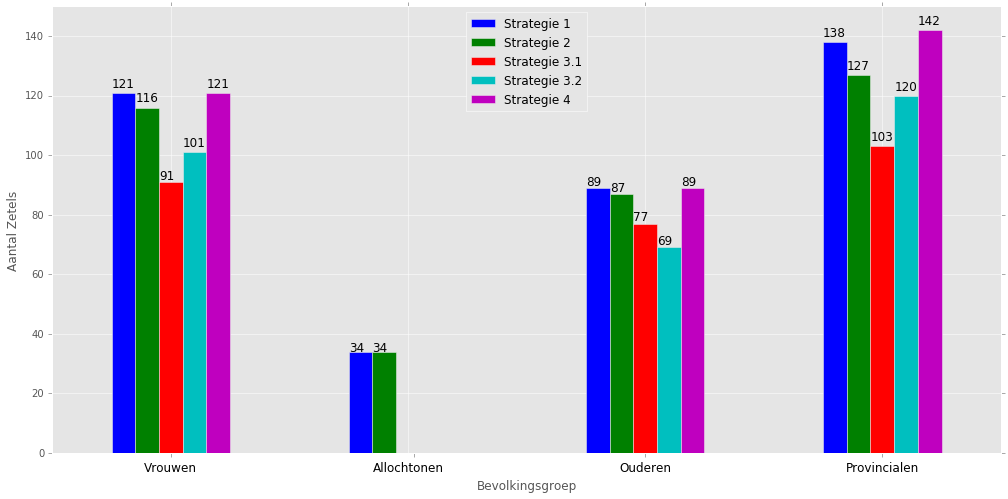
\includegraphics[width=0.95\linewidth]{overzicht_resultaten_strategien_plot.png}

			\caption{Grafiek met overzicht van de resultaten in aantal zetels per strategie en per bevolkingsgroep.}

\label{fig:S_overzicht}
\end{figure}


\subsection{Bevolkingsgroep: Vrouwen.}
\label{vrouwen}
Betreffende de bevolkingsgroep vrouwen in Nederland worden hieronder verschillende strategie\"{e}n uiteengezet. Zodoende pogen we te achterhalen hoe in theorie de meeste vrouwelijke kandidaten in de Tweede Kamer gekozen hadden kunnen worden wanneer alle stemgerechtigde vrouwelijke kiezers in Nederland zich hadden gecommitteerd aan een strategie (zie Bijlage \ref{b1} voor de drie andere bevolkingsgroepen). In Sectie \ref{percV} wordt er onderzocht wat er zou zijn gebeurd wanneer een deel van de bevolkingsgroep zich had gecommitteerd aan een strategie. 

\paragraph{Het berekenen van het aantal te verwachten vrouwelijke stemmen.}
Voor het opzetten van de strategie\"{e}n en het, voor elke strategie, kunnen toewijzen van de stemmen van vrouwelijke kiezers aan de vrouwelijke kandidaten van de partijen moeten we eerst weten hoeveel stemmen de partijen volgens de peiling zou gaan ontvangen. Dit doen we door de verwachte opkomst te delen door het aandeel zetels(in een percentage) dat een partij volgens de peiling zal ontvangen. Ter illustratie het volgende voorbeeld: In de peiling van 11 september 2012 \citep{IPSOS} werd er een opkomst van 73\% van alle stemgerechtigden verwacht. Er waren in 2012 een totaal aantal van 12.689.810 stemgerechtigden \citep{Kiesraad_uitslag}. Dat betekent dat 73\% van alle stemgerechtigden uitkomt op (0,73*12.689.810 = ) 9.263.561 te verwachten stemmen. Het aantal stemmen die een partij zou gaan ontvangen is dus het aandeel van het aantal zetels in de Tweede Kamer dat een partij zou gaan ontvangen volgens de peiling. Ter illustratie het volgende voorbeeld: de PVDA  zou, volgens de peiling,  36 zetels ontvangen. Dat komt neer op een percentage van (36/150 zetels = ) 24\% van alle zetels. Het aantal stemmen dat de PVDA daarmee zou gaan ontvangen is dan het aantal van (0,24*9.263.561 = ) 2.223.254 stemmen. We nemen aan dat de man-vrouw stemmenverdeling bij elke partij gelijk is. Oftewel de helft van de stemmen die een partij ontvangt komt van mannen en de andere helft van de stemmen komt van vrouwen. Daarmee zal de PVDA het totale aantal van (0,50*2.223.254 = ) 1.111.627 stemmen van vrouwelijke kiezers ontvangen. In Tabel \ref{table:tab1V} hieronder is o.a. te zien hoeveel stemmen de partijen, volgens de peiling, zouden gaan ontvangen van vrouwelijke kiezers. Naast het berekenen van het aantal te verwachten stemmen per partij kunnen we ook de te verwachten voorkeursdrempel berekenen. Zoals eerder al is toegelicht is de voorkeursdrempel 25\% van de kiesdeler. De kiesdeler is het aantal stemmen dat genoeg is voor één zetels. De te verwachten kiesdeler is het aantal van (9.263.561/150 = ) 61.757 stemmen. De te verwachten voorkeursdrempel wordt daarom vastgesteld op het aantal van (0,25*61.757 = ) 15.439 stemmen.






\begin{table}[h]
\centering
	\begin{footnotesize}
		\begin{tabular}{lrr}
\toprule
{} &  Aantal Stemmen Partij &  Aantal Stemmen Van Vrouwen \\
Partij                &                        &                             \\
\midrule
50PLUS                &                 123514 &                       61757 \\
CDA                   &                 741084 &                      370542 \\
ChristenUnie          &                 308785 &                      154392 \\
D66                   &                 679327 &                      339663 \\
GROENLINKS            &                 247028 &                      123514 \\
Partij v d Dieren &                 185271 &                       92635 \\
PVDA                  &                2223254 &                     1111627 \\
PVV                   &                1111627 &                      555813 \\
SGP                   &                 185271 &                       92635 \\
SP                    &                1235141 &                      617570 \\
VVD                   &                2223254 &                     1111627 \\
\bottomrule
\end{tabular}

	\end{footnotesize}
			\caption{Totaal aantal stemmen dat een partij zou gaan ontvangen en het totaal aantal te verwachten vrouwelijke stemmen volgens de peiling \citep{IPSOS}.}
\label{table:tab1V} 
\end{table}

\newpage
\paragraph{Het berekenen van het werkelijke aantal vrouwelijke stemmen.}
Voor het bepalen van het succes van de strategie en het berekenen van het 'werkelijke' aantal stemmen dat een partij van vrouwelijke kiezers zou hebben ontvangen, kijken we eerst naar het totaal aantal stemmen die de partijen volgens de einduitslag hebben ontvangen \citep{Kiesraad_uitslag}. Ook kijken we naar de man-vrouw verdeling van het aantal stemmen op de partijen \citep{IPSOS_man_vrouw}. Ter illustratie het volgende voorbeeld: de PVDA had bij de einduitslag een totaal van 2.340.750 stemmen ontvangen. Hiervan kwamen 52\% van de stemmen van vrouwelijke kiezers. Dit betekent dat de PVDA volgens de einduitslag het aantal van (0.52*2.340.750 = ) 1.217.190 stemmen van vrouwelijk kiezers heeft ontvangen. De vrouwelijke stemmen die een partij heeft ontvangen worden vervolgens willekeurig verdeeld over een \textit{N}  aantal vrouwen. Omdat de \textit{N} aantal vrouwen per strategie en vervolgens per partij telkens anders is wordt er later per strategie aan de hand van voorbeelden uitgelegd hoe de vrouwelijke stemmen die een partij heeft ontvangen worden toegewezen aan de \textit{N} vrouwelijke kandidaten van de partij. Hieronder is tabel \ref{table:tab2V} per partij te zien hoeveel stemmen de partij in totaal heeft ontvangen, hoeveel procent van de stemmen van vrouwelijke kiezers en hoeveel van mannelijk kiezers kwamen en het aantal stemmen dat de partij van vrouwelijke kiezers heeft ontvangen. 


\begin{table}[h]
\centering
	\begin{footnotesize}
		\begin{tabular}{lrrrr} 
\toprule 
{} &  Aantal Stem-  &  Vrouwelijke Stem- &  Mannelijke Stem-  &  Aantal Stemmen  \\
Partij                &        men Partij              &                                men Percentage &            men Percentage                  &    Van Vrouwen                         \\
\midrule
50PLUS                &                 177631 &                              51 &                             49 &                       90591 \\
CDA                   &                 801620 &                              40 &                             60 &                      320648 \\
ChristenUnie          &                 294586 &                              63 &                             37 &                      185589 \\
D66                   &                 757091 &                              42 &                             58 &                      317978 \\
GROENLINKS            &                 219896 &                              48 &                             52 &                      105550 \\
Partij v d Dieren &                 182162 &                              51 &                             49 &                       92902 \\
PVDA                  &                2340750 &                              52 &                             48 &                     1217190 \\
PVV                   &                 950263 &                              44 &                             56 &                      418115 \\
SGP                   &                 196780 &                              51 &                             49 &                      100357 \\
SP                    &                 909853 &                              57 &                             43 &                      518616 \\
VVD                   &                2504948 &                              43 &                             57 &                     1077127 \\
\bottomrule
\end{tabular}

	\end{footnotesize}

			\caption{Totaal aantal stemmen dat een partij heeft ontvangen \citep{Kiesraad_databank} de vrouw-man verdeling van de stemmen in percentages \citep{IPSOS_man_vrouw} en het totaal aantal vrouwelijke stemmen wat de partijen daarmee hebben ontvangen.}
\label{table:tab2V} 
\end{table}




\paragraph{Het uiteindelijk opstellen van de Tweede Kamer na uitvoering van een strategie.}
Nadat bij elke strategie de stemmen van vrouwelijke kiezers per partij zijn toegewezen aan de vrouwelijke kandidaten van de partij moet de nieuwe Tweede Kamer worden opgesteld. Het opstellen van de Tweede Kamer volgt exact de regels
zoals door de Kiesraad \citeyearpar{Kiesraad_voorkeursdrempel2}  worden toegepast
en gaat als volgt: 

\begin{itemize}
	\item
\textbf{Stap 1:} Als eerst wordt er gekeken hoeveel zetels een partij heeft ontvangen bij de uitslag van de Tweede Kamerverkiezingen van 2012. 
	\item
\textbf{Stap 2:} Vervolgens wordt, na toewijzing van de stemmen van vrouwelijke kiezers op vrouwelijke kandidaten, geteld hoeveel kandidaten(mannelijke én vrouwelijke kandidaten) er boven de kiesdrempel uit zijn gekomen. Daarbij moet genoteerd worden dat na uitvoering van de strategie de mannelijke kandidaten evenveel stemmen hebben ontvangen als wanneer de strategie niet wordt uitgevoerd. De reden hiervoor is dat het theoretisch mogelijk is dat de mannelijke kandidaten enkel stemmen hebben ontvangen van mannelijke kiezers. Ook al is dit onwaarschijnlijk, we kunnen dit niet weten en zullen dan ook geen stemmen van de mannelijke kandidaten aftrekken. Derhalve is het aantal stemmen dat een mannelijke kandidaat ontvangt na uitvoering van een strategie hetzelfde als bij de daadwerkelijke verkiezingsuitslag van 2012.
	\item
\textbf{Stap 3:} Nadat we, na uitvoering van een strategie, hebben geteld hoeveel kandidaten genoeg stemmen hebben ontvangen om boven de voorkeursdrempel uit te komen kijken we per partij of de partij een hoger aantal zetels heeft ontvangen dan het aantal kandidaten van de partij die boven de voorkeursdrempel zijn gekomen. 
	\item
\textbf{Stap 4:} Als de partij meer zetels heeft ontvangen dan er voor de partij kandidaten boven de voorkeursdrempel zijn gekomen, worden de resterende zetels vergeven aan de hoogst genoteerde kandidaten op de kandidatenlijst van de partij(mits deze kandidaten dus niet genoeg stemmen hebben ontvangen om boven de voorkeursdrempel uit te komen).
\end{itemize}


\subsubsection*{Beschrijving Strategie\"{e}n} \label{besS}
In deze sectie zullen we vijf strategie\"{e}n worden beschreven waarbij de aannames voor elke strategie hetzelfde zijn. Deze aannames zijn:

\begin{itemize}
	\item 
Alle stemgerechtigde vrouwen waarvan de peiling aangaf dat zij zouden gaan stemmen hebben meegedaan aan de strategie.
	\item
Vrouwelijke kiezers hebben daarbij volstrekt willekeurig gestemd op de top \textit{N} vrouwelijke kandidaten van de partij waar zij toch al op wilden stemmen.	
	\item
Alle stemgerechtigde mannen waarvan de peiling aangaf dat zij zouden gaan stemmen hebben niet meegedaan aan de strategie en hebben ook geen eigen (tegen)strategie bepaald. Mannelijke kiezers hebben derhalve hetzelfde gestemd zoals zij volgens de einduitslag hebben gedaan. 
\end{itemize}


\noindent Voordat we de strategie\"{e}n op de bevolkingsgroep vrouwen gaan toepassen worden hieronder de vijf strategie\"{e}n beknopt beschreven:\\


\newcolumntype{L}{@{}>{\bfseries}p{16em}<{}}% Item label
\newcolumntype{I}{X@{}}% Item contents
\noindent\begin{tabularx}{\textwidth}{LI}
  Strategie 1. Top \textit{N} volgens peiling: & Vrouwelijk kiezers stemmen volstrekt willekeurig op een top \textit{N}  vrouwelijke kandidaat waarbij \textit{N} wordt bepaald door de peiling. \\
  \\
  Strategie 2. Willekeurig: & Vrouwelijke kiezers stemmen volstrekt willekeurig op een vrouwelijke kandidaat.\\
\\
  Strategie 3.1. Top 15: & Vrouwelijke kiezers stemmen volstrekt willekeurig op een van de eerste vrouwelijke kandidaten van de partij \\
\\  
  Strategie 3.2. Top \textit{N} a.d.h.v. aantal vrouwelijke kandidaten: & Vrouwelijke kiezers stemmen volstrekt willekeurig op een van de eerste \textit{N} vrouwelijke kandidaten van de partij waarbij \textit{N} wordt bepaald wordt bepaald door het aantal vrouwelijke kandidaten van de partij.\\
  \\
  Strategie 4. Top \textit{N+extra percentage} volgens peiling: & Vrouwelijke kiezers stemmen volstrekt willekeurig op een top \textit{N} vrouwelijke kandidaat waarbij \textit{N} wordt bepaald door de peiling en een \textit{extra percentage} van \textit{N} die wordt opgeteld bij \textit{N} \\\\
\end{tabularx}




\newpage
\subsubsection{Strategie 1: Vrouwelijke kiezers stemmen volstrekt willekeurig op een top \textit{N} vrouwelijke kandidaat.} \label{S1V}



\paragraph{Regels.}
\begin{itemize}

 		\item
Elke partij krijgt een eigen \textit{N}:
 
		\begin{itemize}
			\item
In het geval de partij minder vrouwen op de kandidatenlijst had staan dan dat de partij, volgens de peiling, aan zetels verwacht werd te gaan ontvangen is \textit{N} gelijk aan het totaal aantal vrouwen op de kandidatenlijst van de partij.
			\item
In het geval de partij meer vrouwelijke kandidaten op de kandidatenlijst had staan dan dat de partij, volgens de peiling, aan zetels zou gaan ontvangen is \textit{N} gelijk aan het totaal aantal zetels die de partij volgens de peiling zou gaan ontvangen.\\	
			
		\end{itemize} 	
\end{itemize} 

\paragraph{Verdelingen zetels en aantal vrouwelijke kandidaten.}
In de grafiek hieronder in Figuur \ref{fig:zetelsV} is te zien dat alle partijen links van de stippellijn hadden meer vrouwelijke kandidaten op de kandidatenlijst \citep{Kiesraad_kandidatenlijsten} hadden staan dan dat zij zetels zouden gaan ontvangen volgens de peiling \citep{IPSOS}. Alle partijen rechts van de stippellijn hadden minder vrouwelijke kandidaten op de kandidatenlijst staan dan dat zij volgens de peiling aan zetels zouden gaan ontvangen. Bij alle partijen links van de stippellijn is \textit{N} daarmee gelijk aan het aantal zetels dat de partij zou gaan ontvangen volgens de peiling. Bij de partijen rechts van de stippellijn is \textit{N} gelijk aan het aantal vrouwelijke kandidaten dat de partij op de kandidatenlijst heeft staan.
 
\begin{figure}[H]

	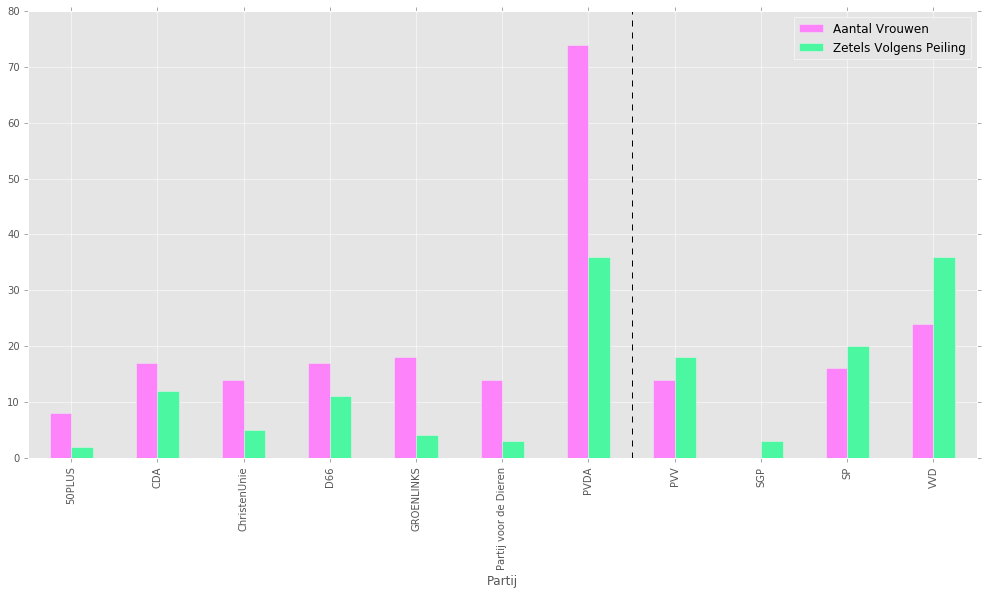
\includegraphics[width=\linewidth]	{Aantal_vrouwen_aantal_zetels.png}

			\caption{Het aantal vrouwen (paarse staven) op de kandidatenlijst \citep{Kiesraad_kandidatenlijsten} en het aantal zetels (groene staven) volgens de peilingen per partij \citep{IPSOS}.}

	\label{fig:zetelsV}
\end{figure}

\paragraph{Maximaal aantal vrouwen per partij (top \textit{N}) dat in de Tweede Kamer gekozen kan worden.}
In Figuur \ref{fig:zetelsV} is te zien hoeveel zetels een partij zou gaan ontvangen volgens de peiling en hoeveel vrouwelijke kandidaten de partij op de kandidatenlijst had staan. In tabel \ref{table:topNV} hieronder is daaruit voortvloeiend te zien hoeveel vrouwelijke kandidaten er per partij maximaal in de Tweede Kamer gekozen hadden kunnen worden.  


\begin{table}[h]
\centering
	\begin{footnotesize}
		\begin{tabular}{lrr}
\toprule
{} &  Top \textit{N} Vrouwelijke Kandidaten  &  Overgebleven Mannelijke Kandidaten  \\
Partij                &        &        \\
\midrule
50PLUS                &                              2 &       0 \\
CDA                   &                             12 &       0 \\
ChristenUnie          &                              5 &       0 \\
D66                   &                             11 &       0 \\
GROENLINKS            &                              4 &       0 \\
Partij v d Dieren &                              3 &       0 \\
PVDA                  &                             36 &       0 \\
PVV                   &                             14 &       4 \\
SGP                   &                              0 &       3 \\
SP                    &                             16 &       4 \\
VVD                   &                             24 &      12 \\
\midrule
Totaal                &                            127 &      23 \\
\bottomrule
\end{tabular}

	\end{footnotesize}
			\caption{Per partij de top \textit{N} vrouwelijke kandidaten en de overgebleven mannelijke kandidaten a.d.h.v. de peiling \citep{IPSOS}.}
\label{table:topNV} 
\end{table}

Vanwege het feit dat de SGP helemaal geen vrouwelijke kandidaten op de kandidatenlijst had staan en de PVV, de SP en de VVD volgens de peiling meer zetels zouden gaan ontvangen dan dat zij vrouwelijke kandidaten op de kandidatenlijsten hadden staan komt het totaal aantal vrouwelijke kandidaten dat volgens de peiling in de Tweede Kamer gekozen had kunnen worden uit op 127. De overgebleven 23 kandidaten die op basis van de peiling in de Tweede Kamer zouden worden gekozen, zijn uiteraard mannelijke kandidaten.

\paragraph{Het toewijzen van de stemmen aan de vrouwelijke kandidaten op basis van de peiling.}
Zoals te zien in Tabel \ref{table:tab1V}, hebben we berekend hoeveel stemmen een partij, volgens de peiling, werd verwacht te gaan ontvangen en hoeveel stemmen van vrouwelijke kiezers een partij verwacht werd te gaan ontvangen. Nu gaan we deze vrouwelijke stemmen toewijzen aan vrouwelijke kandidaten op de kandidatenlijsten. De reden hiervoor is dat er zodoende een voorspelling gedaan kan worden over het aantal stemmen dat de top \textit{N} vrouwelijke kandidaten van een partij per vrouwelijke kandidaat kon gaan verwachten. Ter illustratie nemen we weer de PVDA als voorbeeld.

Voor de PVDA werd verwacht dat zij een totaal aantal van 1.111.627 vrouwelijke stemmen zouden gaan ontvangen. Deze stemmen worden verdeeld over de top \textit{N} vrouwelijke kandidaten van de PVDA. Zoals eerder al vastgesteld, en te zien in Tabel \ref{table:topNV}, heeft de PVDA een \textit{N} = 36. De stemmen van vrouwelijke kiezers op de PVDA worden willekeurig (gelijk) verdeeld over de eerste 36 vrouwelijke kandidaten op de kandidatenlijst van de PVDA. Daarmee krijgen de top 36 vrouwelijke kandidaten van de PVDA (ongeveer) het aantal van (1.111.627/36 = ) 30.878 stemmen per top \textit{N} vrouwelijke kandidaat. Dat is ruim boven de verwachte voorkeursdrempel van het aantal van 15.439 stemmen. In de grafiek in Figuur \ref{fig:stemmenV1} is, gebaseerd op de peiling, de verdeling van vrouwelijke stemmen op vrouwelijke kandidaten voor alle partijen te zien.

  
\begin{figure}[H]

	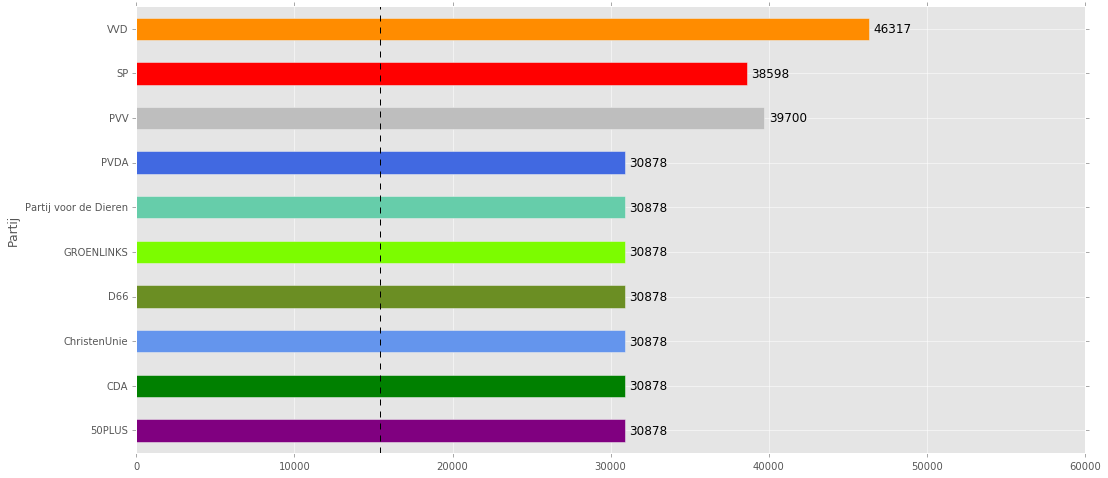
\includegraphics[width=\linewidth]	{stemmen_op_vrouwen_topN_peiling.png}

			\caption{Grafiek met per partij met vrouwelijke kandidaten, de verdeling van de stemmen van vrouwelijk kiezers op de top \textit{N} vrouwelijke kandidaten aan de hand van de peiling \citep{IPSOS}. De stippellijn is de verwachte voorkeursdrempel(15.439 stemmen).}

\label{fig:stemmenV1}
\end{figure}

Zoals te zien in Figuur \ref{fig:stemmenV1} hierboven, kan volgens de peiling voor alle top \textit{N} vrouwelijke kandidaten verwacht worden dat zij boven de verwachte voorkeursdrempel uitkomen. Hierdoor zou het mogelijk zijn geweest dat alle 127 top \textit{N} vrouwelijke kandidaten in de Tweede Kamer gestemd konden worden. Wat opvalt is dat voor zeven verschillende partijen het aantal te verwachten stemmen op een vrouwelijke kandidaat van de partijen exact hetzelfde is. Dit is geen toeval maar ligt ten grondslag aan de manier van berekenen.

De partijen waarbij het aantal stemmen op een top \textit{N} vrouwelijke kandidaat hetzelfde is, hebben allemaal één ding gemeen: de top \textit{N} is gelijk aan het aantal te verwachten zetels. Zoals eerder al is uitgelegd, is het aantal stemmen dat nodig is voor één te verwachte zetel gelijk aan de verwachte kiesdeler (61.757 stemmen). Vanwege de aanname dat 50\% van de stemmen op een partij van vrouwelijke kiezers zal komen, wordt de kiesdeler vermenigvuldigd met 50\%. In het geval dat een partij bijvoorbeeld één zetel verwachtte te gaan ontvangen, is het aantal stemmen dat voor deze partij werd verwacht gelijk aan de verwachte kiesdeler. Wanneer 50\% van de stemmen van vrouwelijk kiezers zou zijn gekomen en van deze kiezers verwacht werd dat zij allemaal op de enige mogelijke vrouwelijke kandidaat zouden hebben gestemd (voor deze partij geldt dan \textit{N=1}), zou deze vrouwelijke kandidaat het verwachte aantal van ($50\%*61.757$ = ) 30.878 stemmen hebben ontvangen. 


\paragraph{Het toewijzen van de stemmen aan de vrouwelijke kandidaten op basis van einduitslag.}
In de vorige paragraaf werd uitgelegd hoe we, aan de hand van de peiling, een voorspelling konden gaan doen over het aantal stemmen dat een top \textit{N} vrouwelijke kandidaat kon gaan verwachten. Zoals te zien in Tabel \ref{table:tab2V} en zoals we eerder in dit hoofdstuk hebben berekend, weten we hoeveel stemmen van vrouwelijke kiezers een partij volgens de einduitslag heeft ontvangen. Zodoende kunnen we het aantal stemmen van vrouwelijke kiezers gaan toewijzen aan de vrouwelijke kandidaten en kunnen we daarmee gaan bepalen of de voorspelling uit de vorige paragraaf enigszins correct is. Ter illustratie nemen we weer de PVDA als voorbeeld. \\
\indent De PVDA heeft bij de einduitslag een totaal aantal van 1.217.190 aantal vrouwelijke stemmen ontvangen. Deze stemmen worden willekeurig verdeeld over de top 36 (voor de PVDA geldt \textit{N} = 36) vrouwelijke kandidaten van de PVDA. Daarmee zouden de deze vrouwelijke kandidaten van de PVDA het aantal van ($1.217.190\div36$ = ) 33.810 stemmen per kandidaat hebben ontvangen. Dat is ruim boven de daadwerkelijke voorkeursdrempel van 15.708 stemmen. In de grafiek in Figuur \ref{fig:stemmenV2} is, gebaseerd op de einduitslag, de verdeling van vrouwelijke stemmen op vrouwelijke kandidaten voor alle partijen te zien.

  
\begin{figure}[H]

	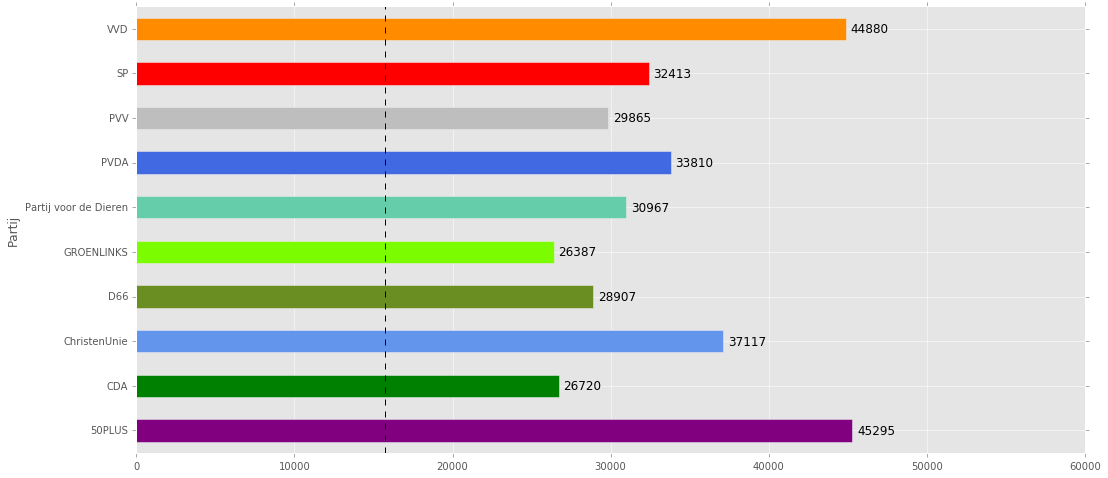
\includegraphics[width=\linewidth]	{stemmen_op_vrouwen_topN_uitslag.png}

			\caption{Grafiek met per partij de verdeling van de stemmen van vrouwelijk kiezers op de top \textit{N} vrouwelijke kandidaten aan de hand van de einduitslag \citep{Kiesraad_databank}. De SGP wordt niet in de grafiek getoond omdat deze partij geen vrouwelijke kandidaten op de kandidaten lijst heeft staan. De stippellijn is de daadwerkelijke voorkeursdrempel(15.708 stemmen).}

\label{fig:stemmenV2}
\end{figure}

Zoals te zien in Figuur \ref{fig:stemmenV2} hierboven, zouden alle top \textit{N} vrouwelijke kandidaten van de partijen boven de daadwerkelijke voorkeursdrempel uitgekomen zijn. Ofschoon de precieze aantallen niet exact hetzelfde zijn, is de voorspelling uit de vorige paragraaf correct in het feit dat de top \textit{N} vrouwelijke kandidaten van alle partijen boven de voorkeursdrempel uitgekomen zouden zijn. Het is op basis van de einduitslag nog altijd mogelijk dat er 127 vrouwelijke kandidaten in de Tweede Kamer worden gekozen. 

\paragraph{Aantal vrouwen na strategie 1.}
Na het uitvoeren van de strategie 1 en het opstellen van de Tweede Kamer zoals eerder in dit hoofdstuk beschreven (zie paragraaf \hyperref[opstellen]{Het uiteindelijk opstellen van de Tweede Kamer na uitvoering van een strategie.}), zou strategie 1 een Tweede Kamer hebben opgeleverd waarin 121 vrouwen en 29 mannen plaatsnemen. Daarmee zouden vrouwen (met 81\%) ruim in hogere mate vertegenwoordigd zijn dan mannen (met 19\%). In de cirkeldiagram in Figuur \ref{fig:pcS1V} hieronder is de verdeling goed te zien. In de volgende paragraaf wordt uitgelegd waarom er niet 127 maar 'slechts' 121 vrouwen in de Tweede Kamer plaats zouden nemen na uitvoering van strategie 1.

\begin{figure}[H]
\centering
	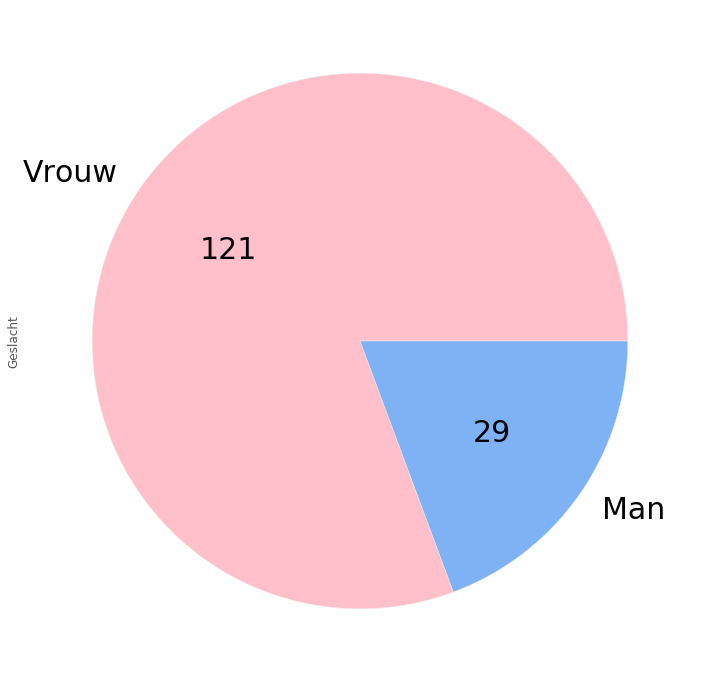
\includegraphics[width=0.35\linewidth]{pie_chart_topN.png}

			\caption{Na uitvoering van de strategie nemen er 121 vrouwen(81\%) en 29 mannen(19\%) plaats in de Tweede Kamer.}

\label{fig:pcS1V}
\end{figure}

\paragraph{Minder vrouwen dan 127 vrouwen in de Tweede Kamer na uitvoering van strategie 1.}
De reden dat er niet 127 vrouwen maar 'slechts' 121 vrouwen in de Tweede Kamer plaatsnemen na uitvoering van strategie 1 ligt ten grondslag aan een aantal factoren. Zo hadden het merendeel van de partijen die zetels ontvingen een mannelijke kandidaat als lijsttrekker en ontvingen deze lijsttrekkers de meeste stemmen in vergelijking met alle andere kandidaten van dezelfde partij. Hierdoor viel er uiteindelijk bij zowel de 50PLUS, de ChristenUnie als de SP één vrouwelijke kandidaat af. Daarnaast had de SP minder zetels behaald bij de einduitslag dan zij volgens de peiling zou gaan ontvangen. Hierdoor viel ook bij de SP nog een vrouwelijke kandidaat af. Ook de Partij voor de Dieren ontving minder zetels bij de einduitslag dan zij volgens de peiling zouden gaan ontvangen en, ondanks het feit dat zij een vrouwelijke lijsttrekker hadden in de persoon van Marianne Thieme, resulteerde dit in één afgevallen vrouwelijke kandidaat. Bij het CDA had een mannelijke kandidaat in de persoon van Pieter Omtzigt meer stemmen ontvangen dan de vrouwelijke kandidaten. Hierdoor viel bij het CDA een vrouwelijke kandidaat af. Dit komt op een totaal van zes afgevallen vrouwelijke kandidaten, oftewel een totaal van (127 - 6 = ) 121 vrouwen in de Tweede Kamer na uitvoering van strategie 1.  



\subsubsection{Strategie 2: Vrouwelijke kiezers stemmen op een willekeurige vrouwelijke kandidaat.}
\paragraph{Regels.}
\begin{itemize}
	\item
Het aantal stemmen van vrouwelijke kiezers die een partij krijgt, worden volstrekt willekeurig verdeeld over het alle vrouwelijke kandidaten die op de kandidatenlijst staan van de partij. Hierbij is \textit{N} per partij het totaal aantal vrouwelijke kandidaten die de partij op de kandidatenlijst heeft staan. 	\\ 	
\end{itemize}	

\paragraph{Het toewijzen van de stemmen aan de vrouwelijke kandidaten op basis van de peiling en de einduitslag.}
Zoals we bij de vorige strategie hebben gedaan, zullen we ook voor strategie 2 de stemmen toewijzen om aan de hand van de peiling een voorspelling te kunnen doen betreffende het aantal te stemmen die per vrouwelijke kandidaat verwacht kan worden. Om te kijken of de voorspelling enigszins correct is en om te weten van welke partijen de vrouwelijke kandidaten in 'werkelijkheid' boven de daadwerkelijke voorkeursdrempel uitkomen, zullen we ook de stemmen op vrouwelijke kandidaten op basis van de einduitslag toewijzen. In Figuur \ref{fig:stemmenS2V}  hieronder is zowel de toewijzing op basis van de peiling alsmede de toewijzing op basis van de einduitslag te zien.   



\begin{figure}[H]

	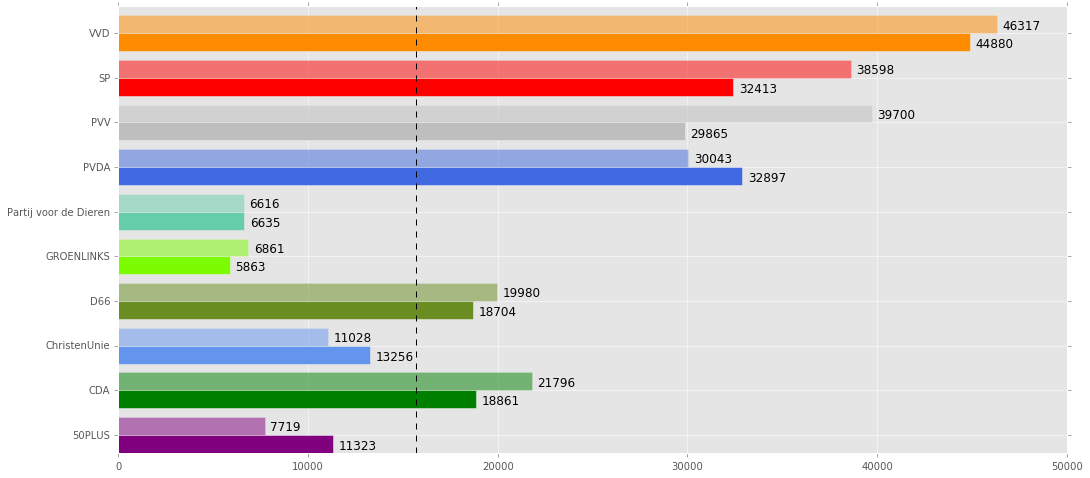
\includegraphics[width=\linewidth]	{stemmen_op_vrouwen_willekeurig_samen.png}

			\caption{Grafiek met per partij de verdeling van de stemmen van vrouwelijk kiezers op alle vrouwelijke kandidaten van de partij a.d.h.v. de peiling (licht gekleurd) en a.d.h.v. de einduitslag (donker gekleurd). De stippellijn is de daadwerkelijk voorkeursdrempel(15.708 stemmen).}

\label{fig:stemmenS2V}
\end{figure}


Zoals te zien in Figuur \ref{fig:stemmenS2V}  hierboven, zijn zowel volgens de peiling (voorspelling) alsmede volgens de einduitslag niet alle vrouwelijke kandidaten van de partijen boven de daadwerkelijke voorkeursdrempel uitgekomen. Ofschoon de precieze aantallen niet exact hetzelfde zijn, is met strategie 2 de voorspelling zoals berekend a.d.h.v. de peiling correct in het voorspellen welke partijen met alle vrouwelijke kandidaten boven de voorkeursdrempel uitkomen en welke partijen dit niet het geval is.




\paragraph{Aantal vrouwen na strategie 2.}
Na het uitvoeren van de strategie 2 en het opstellen van de Tweede Kamer zoals eerder in dit hoofdstuk beschreven (zie paragraaf Het uiteindelijk opstellen van de Tweede Kamer na uitvoering van een strategie.), levert strategie 2 uiteindelijk een Tweede Kamer op waarin 116 vrouwen en 34 mannen plaatsnemen. Daarmee zijn vrouwen(met 77\%) ruim in hogere mate vertegenwoordigd dan mannen(met 23\%). In de cirkeldiagram in Figuur \ref{fig:pcS2V} hieronder is de verdeling goed te zien. In de volgende paragraaf wordt uitgelegd waarom er niet 121 (zoals in de vorige strategie) maar 'slechts' 116 vrouwen in de Tweede Kamer plaatsnemen na uitvoering van strategie 2 ten opzichte van strategie 1.

\begin{figure}[H]
\centering
	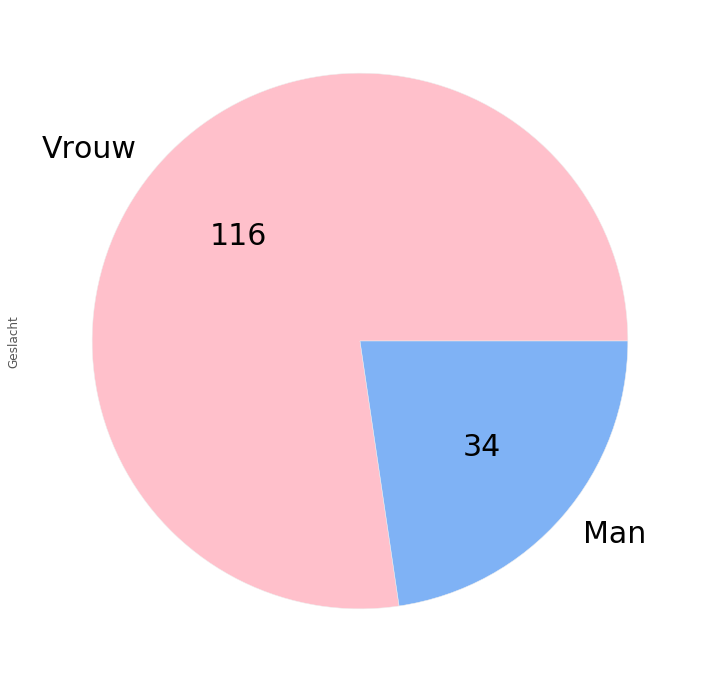
\includegraphics[width=0.35\linewidth]{pie_chart_willekeurig.png}

			\caption{Na uitvoering van de strategie nemen er 116 vrouwen(77\%) en 34 mannen(23\%) plaats in de Tweede Kamer.}

\label{fig:pcS2V}
\end{figure}

\paragraph{Minder vrouwen in de Tweede Kamer d.m.v. uitvoering van strategie 2 dan d.m.v. uitvoering van strategie 1.}
De reden dat er, na uitvoering van strategie 2, 116 vrouwen in de Tweede Kamer plaatsnemen en dat vijf vrouwen minder zijn dan bij strategie 1 ligt ten grondslag aan het feit dat de vrouwelijke kandidaten van de Partij voor de Dieren, GROENLINKS, de ChristenUnie en 50PLUS minder stemmen ontvangen dan de voorkeursdrempel. Bij de Partij voor de Dieren heeft dit echter geen negatief effect vanwege het feit dat de partij twee zetels ontvangt en de eerste twee plaatsen op de kandidatenlijst worden bezet door vrouwelijke kandidaten. Bij zowel GROENLINKS alsmede de ChristenUnie vallen er echter twee vrouwelijke kandidaten af. Bij 50PLUS valt er één vrouwelijke kandidaat af. Geen enkele partij krijgt meer vrouwen in de Tweede Kamer na uitvoering van strategie 2 ten opzichte van strategie 1.   


\subsubsection{Strategie 3.1: Vrouwelijke kiezers stemmen willekeurige op één van de eerste 15 vrouwelijke kandidaten van een partij.}

\paragraph{Regels.}
\begin{itemize}
\item
Elke partij krijgt een eigen \textit{N}:
	\begin{itemize}
		\item
Wanneer een partij 15 of meer vrouwelijke kandidaten op de kandidatenlijst heeft staan geldt voor de partij 	\textit{N} = 15.
		\item
Wanneer een partij minder dan 15 vrouwelijke kandidaten op de kandidatenlijst heeft staan, geldt voor de partij \textit{N} = het totaal aantal vrouwelijke kandidaten wat de partij op de kandidatenlijst heeft staan.\\
	\end{itemize}
\end{itemize}

\paragraph{Partijen met minstens 15 vrouwelijke kandidaten en partijen met minder dan 15 vrouwelijke kandidaten.}
Hieronder is in de grafiek in Figuur \ref{fig:15V} per partij te zien of de partij voldoet aan de drempel van minstens 15 vrouwelijke kandidaten op de kandidatenlijst om de zodoende de vrouwelijke stemmen op de partij te gaan verdelen over de top 15 vrouwelijke kandidaten van de partij. We zien dat bij D66, GROENLINKS, de PVDA, het CDA, de SP en de VVD de stemmen van vrouwelijke kiezers over de top 15 vrouwelijke kandidaten verdeeld kunnen worden. Bij de Partij voor de Dieren, de ChristenUnie, 50PLUS en de PVV moeten de stemmen van vrouwelijke kiezers die de partij volgens de peiling zou gaan ontvangen verdeeld worden over alle vrouwelijke kandidaten die deze partijen op hun kandidatenlijsten hadden staan.

\begin{figure}[H]

	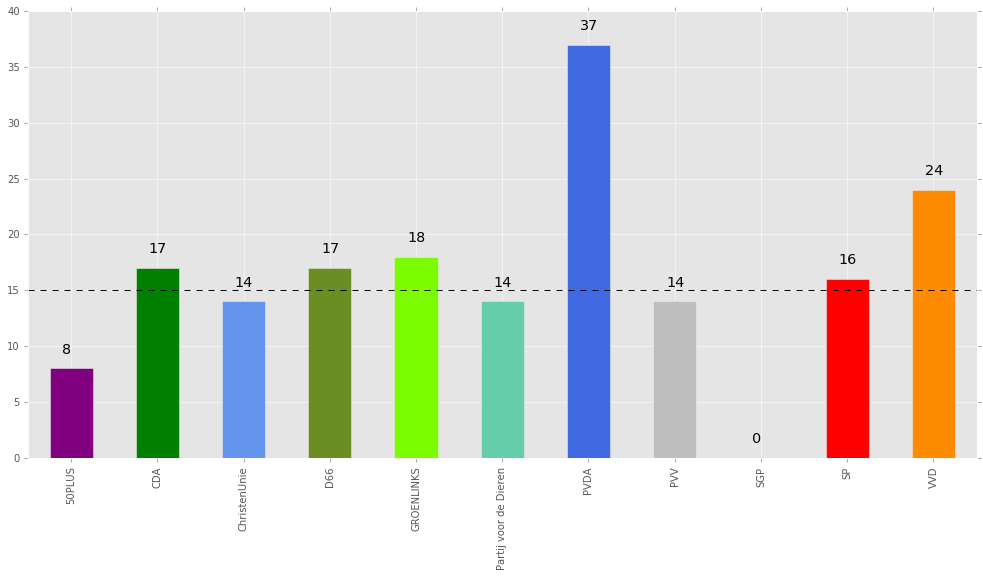
\includegraphics[width=\linewidth]	{top15_of_topN_kandidaten.png}

			\caption{De grafiek toont bij welke partijen de vrouwelijke kiezers op de top 15 vrouwelijke kandidaten van de partij kunnen gaan stemmen (\textit{N=15}) en van welke partijen de vrouwelijke kiezers op alle vrouwelijke kandidaten van de partij kunnen gaan stemmen (\textit{N=totaal aantal vrouwelijke kandidaten}).}  

\label{fig:15V}
\end{figure}

\paragraph{Het toewijzen van de stemmen aan de vrouwelijke kandidaten op basis van de peiling.}
Zoals te zien in Tabel \ref{table:tab1V}, hebben we berekend hoeveel stemmen een partij, volgens de peiling, verwacht werd te gaan ontvangen en hoeveel stemmen van vrouwelijke kiezers een partij verwacht werd te gaan ontvangen. Nu gaan we de vrouwelijke stemmen toewijzen aan vrouwelijke kandidaten op de kandidatenlijsten. 

Op dezelfde wijze als we bij de vorige strategie hebben gehanteerd zullen we ook voor strategie 3 de stemmen toewijzen om a.d.h.v. de peiling een voorspelling te kunnen doen betreffende het aantal stemmen dat per vrouwelijke kandidaat verwacht kan worden. Om de voorspelling te evalueren en om te weten van welke partijen de top \textit{N} vrouwelijke kandidaten in 'werkelijkheid' boven de voorkeursdrempel uitkomen, zullen we ook de stemmen op vrouwelijke kandidaten op basis van de einduitslag toewijzen. In Figuur \ref{fig:stemmenS31V} hieronder is zowel de toewijzing op basis van de peiling alsmede de toewijzing op basis van de einduitslag te zien.  



\begin{figure}[H]

	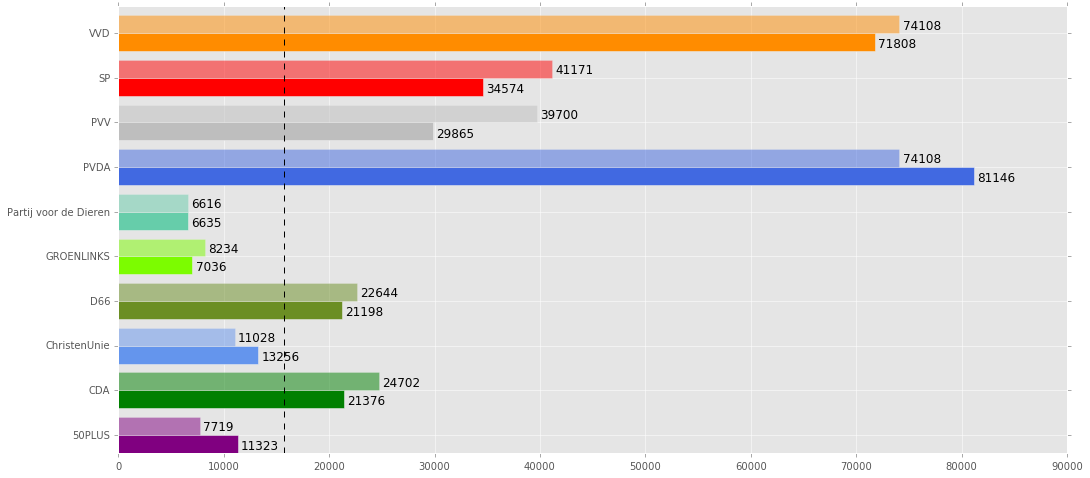
\includegraphics[width=\linewidth]	{stemmen_op_vrouwen_top15_of_topN_samen.png}

			\caption{Grafiek met per partij de verdeling van de stemmen van vrouwelijk kiezers op alle vrouwelijke kandidaten van de partij a.d.h.v. de peiling (licht gekleurd) en a.d.h.v. de einduitslag (donker gekleurd). De stippellijn is de daadwerkelijk voorkeursdrempel(15.708 stemmen).}

\label{fig:stemmenS31V}
\end{figure}

In Figuur \ref{fig:stemmenS31V} hierboven, zijn zowel volgens de peiling (voorspelling) alsmede volgens de einduitslag niet alle top \textit{N} vrouwelijke kandidaten van de partijen boven de daadwerkelijke voorkeursdrempel uitgekomen. Ofschoon de precieze aantallen niet exact hetzelfde zijn, is ook met strategie 3 de voorspelling zoals berekend a.d.h.v. de peiling correctvoorspellen welke partijen met de top \textit{N} (\textit{N=15} of \textit{N=totaal aantal vrouwelijke kandidaten}) vrouwelijke kandidaten boven de voorkeursdrempel uitkomen en van welke partijen dit niet het geval is.


\paragraph{Aantal vrouwen na strategie 3.1.}
Na het uitvoeren van de strategie 3.1 en het opstellen van de Tweede Kamer zoals eerder in dit hoofdstuk beschreven, levert strategie 3.1 uiteindelijk een Tweede Kamer op waarin waarin 91 vrouwen en 59 mannen plaatsnemen. Daarmee zijn vrouwen(met 61\%) in hogere mate vertegenwoordigd dan mannen(met 39\%). In de cirkeldiagram in Figuur \ref{fig:pcS31V} hieronder is de verdeling goed te zien. In de volgende paragraaf wordt uitgelegd waarom er niet 116 (zoals in de vorige strategie) maar slechts 91 vrouwen in de Tweede Kamer Plaatsnemen na uitvoering van strategie 3.1 ten opzichte van strategie 2.

\begin{figure}[H]
\centering
	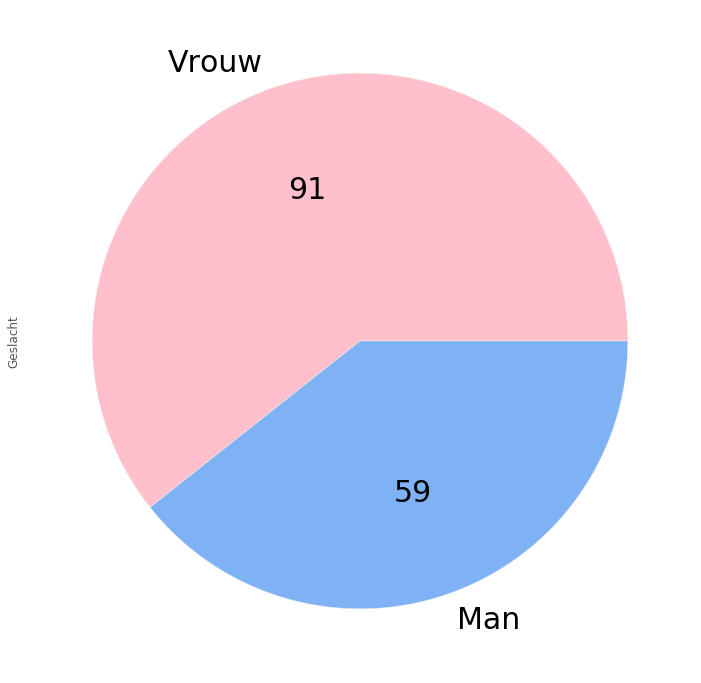
\includegraphics[width=0.35\linewidth]{pie_chart_top15_of_topN.png}

			\caption{Na uitvoering van de strategie nemen er 91 vrouwen(61\%) en 59 mannen(39\%) plaats in de Tweede Kamer.}

\label{fig:pcS31V}
\end{figure}

\paragraph{Minder vrouwen in de Tweede Kamer d.m.v. uitvoering van strategie 3.1 dan d.m.v. uitvoering van strategie 2.}
De reden dat er, na uitvoering van strategie 3.1, 91 vrouwen in de Tweede Kamer plaatsnemen en dat er daarmee 25 vrouwen minder plaatsnemen in de Tweede Kamer dan bij strategie 2 het geval zou zijn, ligt ten grondslag aan het feit dat er bij de VVD 8 vrouwelijke kandidaten afvallen ten opzichte van strategie 2. Dit komt omdat de stemmen niet verdeeld worden over alle 24 vrouwelijke kandidaten van de VVD maar over de top 15 vrouwelijke kandidaten van de VVD. De top 15 vrouwelijke kandidaten van de VVD ontvangen daardoor allen een zetel in de Tweede Kamer. Daarnaast ontvangt ook een 16e vrouwelijke kandidaat, in de persoon van Ingrid de Caluwé, een zetel in de Tweede Kamer vanwege haar plaats op de kandidatenlijst. Ook vallen er bij de PVDA 17 vrouwelijke kandidaten af. Dit komt ook hier door het feit dat er de vrouwelijke stemmen verdeeld worden over de top 15 vrouwelijke kandidaten. Daarnaast ontvangen vier vrouwelijke kandidaten van de PVDA een zetel in de Tweede Kamer vanwege hun plaats op de kandidatenlijst. In totaal vallen er dus 25(17 van de PVDA en 8 van de VVD) vrouwen buiten de boot na uitvoering van strategie 3.1 ten opzichte van strategie 2. Daarmee komt het totale aantal vrouwen in de Tweede Kamer uit op ($116-25$ = ) 91. 



\subsubsection{Strategie 3.2: Vrouwelijke kiezers stemmen willekeurige op één van de eerste \textit{N} vrouwelijke kandidaten van een partij.}

\paragraph{Regels.}
\begin{itemize}
\item
Elke partij krijgt een eigen \textit{N}:

	\begin{itemize}
		\item
Wanneer een partij minder dan 10 vrouwelijke kandidaten op de kandidatenlijst heeft staan geldt voor de partij \textit{N=5} .
		\item
Wanneer een partij tussen de 10 en (minder dan) 15 vrouwelijke kandidaten op de kandidatenlijst heeft staan geldt voor de partij \textit{N=10}.
		\item
Wanneer een partij tussen de 15 en (minder dan) 30 vrouwelijke kandidaten op de kandidatenlijst heeft staan geldt voor de partij \textit{N=15} .
		\item
Wanneer een partij 30 of meer vrouwelijke kandidaten op de kandidatenlijst heeft staan geldt voor de partij \textit{N=30}.
	\end{itemize}
\end{itemize}


\paragraph{Voor elke partij de eigen \textit{N} bepalen.}
Hieronder is in de grafiek in Figuur \ref{fig:XV} per partij te zien op welke waarde het \textit{N} vrouwelijke kandidaten wordt bepaald. De SGP heeft geen vrouwelijke kandidaten op de kandidaten lijst dus de SGP krijgt geen eigen \textit{N}. 50PLUS heeft minder dan 10 vrouwelijke kandidaten op de kandidatenlijst en daardoor wordt geldt voor 50PLUS \textit{N=5}. De ChristenUnie, de Partij voor de Dieren en de PVV hebben 10 of meer vrouwelijke kandidaten op de kandidatenlijsten maar minder dan 15. Hierdoor geldt voor deze partijen \textit{N=10}. Het CDA, D66, GROENLINKS, de SP en de VVD hebben 15 of meer vrouwelijke kandidaten op de kandidatenlijsten maar minder dan 30. Hierdoor geldt voor deze partijen \textit{N=30}. Enkel de PVDA heeft meer dan 30 vrouwelijke kandidaten op de kandidatenlijst staan en daardoor geldt voor de PVDA \textit{N=30}.

\begin{figure}[H]

	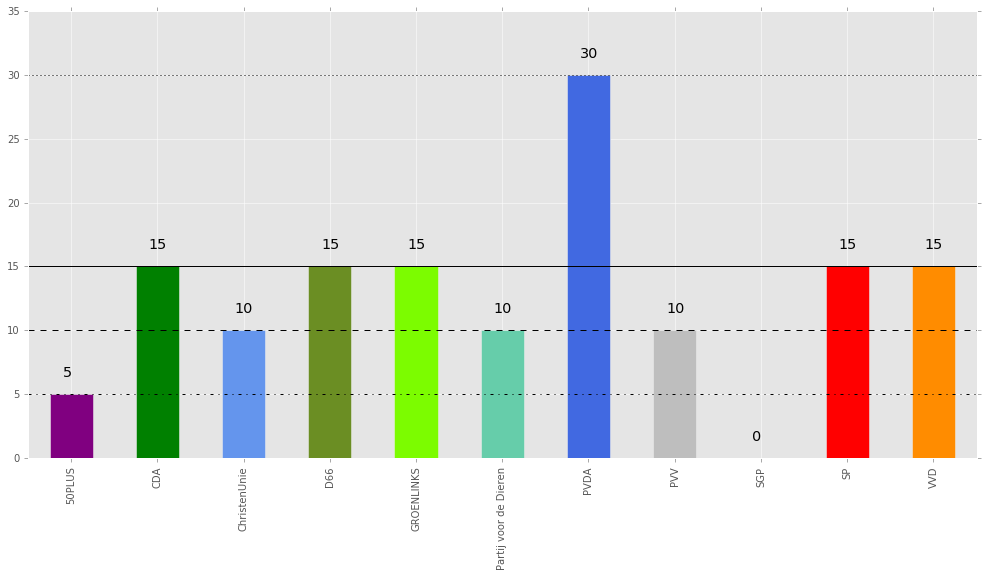
\includegraphics[width=\linewidth]{eigenX_partijen.png}

			\caption{Elke partij krijgt een eigen \textit{X}. De lijnen geven een verschillende mogelijk \textit{X} aan.}

\label{fig:XV}
\end{figure}

\paragraph{Het toewijzen van de stemmen aan de vrouwelijke kandidaten op basis van de peiling.}
Zoals te zien in Tabel \ref{table:tab1V} hebben we berekend hoeveel stemmen een partij volgens de peiling verwacht werd te gaan ontvangen en hoeveel stemmen van vrouwelijke kiezers een partij verwacht werd te gaan ontvangen. Nu gaan we de vrouwelijke stemmen toewijzen aan vrouwelijke kandidaten op de kandidatenlijsten. Op dezelfde wijze als bij de voorgaande strategie\"{e}n hebben gehanteerd zullen we ook voor strategie 3.2 de stemmen toewijzen om a.d.h.v. de peiling een  voorspelling te kunnen doen betreffende het aantal stemmen dat per vrouwelijke kandidaat verwacht kan worden. Om de voorspelling te evalueren en om te weten van welke partijen de top \textit{N} vrouwelijke kandidaten in 'werkelijkheid' boven de voorkeursdrempel uitkomen, zullen we ook de stemmen op vrouwelijke kandidaten op basis van de einduitslag toewijzen. In Figuur \ref{fig:stemmenS32V}  hieronder is zowel de toewijzing op basis van de peiling alsmede de toewijzing op basis van de einduitslag te zien.  




\begin{figure}[H]

	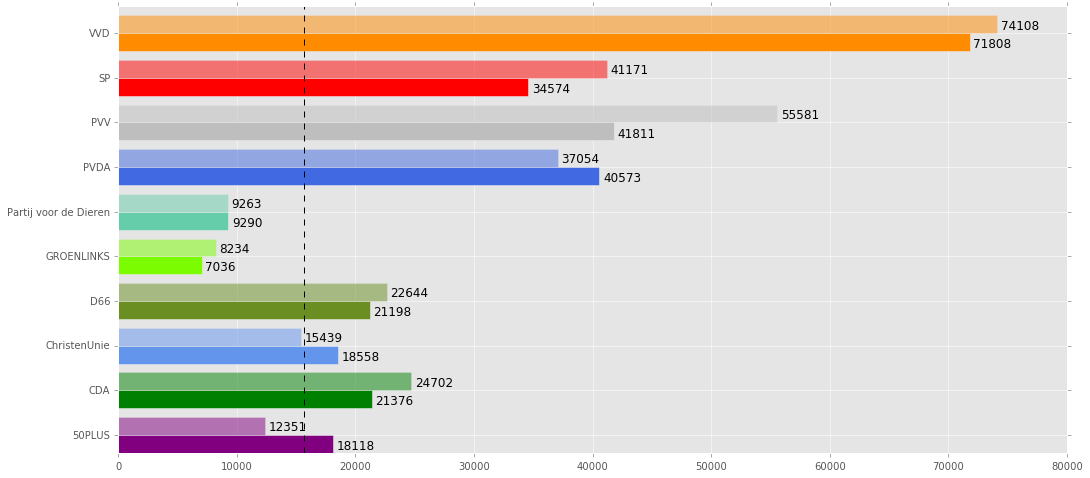
\includegraphics[width=\linewidth]{stemmen_op_vrouwen_eigenX_samen.png}

			\caption{Grafiek met per partij de verdeling van de stemmen van vrouwelijk kiezers op alle vrouwelijke kandidaten van de partij a.d.h.v. de peiling (licht gekleurd) en a.d.h.v. de einduitslag (donker gekleurd). De stippellijn is de daadwerkelijk voorkeursdrempel(15.708 stemmen).}

\label{fig:stemmenS32V}
\end{figure}


In Figuur \ref{fig:stemmenS32V} hierboven, zijn zowel volgens de peiling (voorspelling) alsmede volgens de einduitslag niet alle top \textit{N} vrouwelijke kandidaten van de partijen boven de daadwerkelijke voorkeursdrempel uitgekomen. Ofschoon de precieze aantallen niet exact hetzelfde zijn, is met strategie 3.2 de voorspelling zoals berekend a.d.h.v. de peiling grotendeels correct in het voorspellen welke partijen met de top \textit{N}  vrouwelijke kandidaten boven de voorkeursdrempel uitkomen en van welke partijen dit niet het geval is. Echter is er voor de ChristenUnie verwacht dat de top tien vrouwelijke kandidaten (voor ChristenUnie geldt \textit{N=10}) boven de voorkeursdrempel uit zouden komen terwijl dit bij de einduitslag niet het geval blijkt te zijn. Dit ligt ten grondslag aan het feit dat de ChristenUnie een kleiner aantal stemmen kreeg dan de peiling had voorspeld. Zij kregen derhalve minder stemmen per zetel (58.917 stemmen) dan de daadwerkelijke hoogte van de kiesdeler (62.829 stemmen). 

\paragraph{Aantal vrouwen na strategie 3.2.}
Na het uitvoeren van de strategie 3.2 en het opstellen van de Tweede Kamer zoals eerder in dit hoofdstuk beschreven, levert strategie 3.2 uiteindelijk een Tweede Kamer op waarin waarin 101 vrouwen en 49 mannen plaatsnemen. Daarmee zijn vrouwen(met 67\%) in hogere mate vertegenwoordigd dan mannen(met 33\%). In de cirkeldiagram in Figuur \ref{fig:pcS32V} hieronder is de verdeling goed te zien. In de volgende paragraaf wordt uitgelegd waarom er een toename is van 91 naar 101 vrouwen die in de Tweede Kamer plaatsnemen na uitvoering van strategie 3.2 ten opzicht van strategie 3.1.

\begin{figure}[H]
\centering
	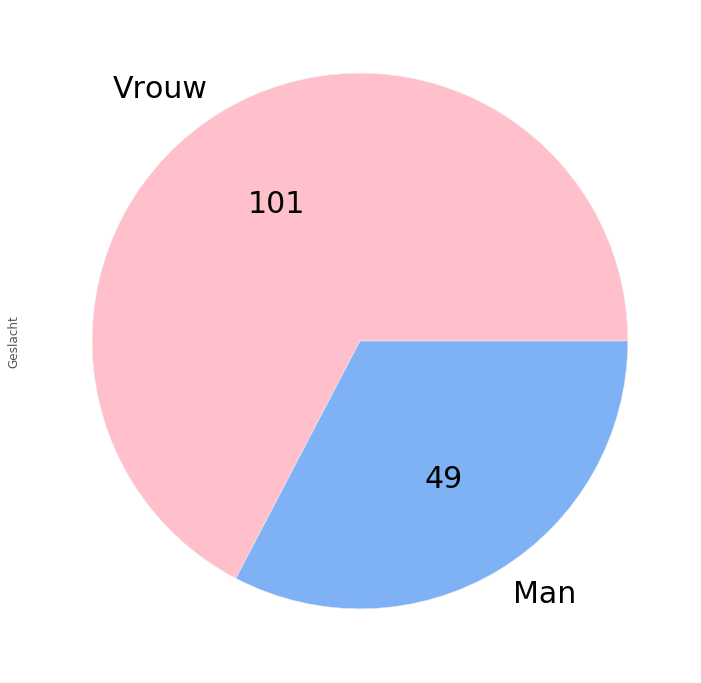
\includegraphics[width=0.35\linewidth]{pie_chart_eigenX.png}

			\caption{Na uitvoering van de strategie nemen er 101 vrouwen(67\%) en 49 mannen(33\%) plaats in de Tweede Kamer.}

\label{fig:pcS32V}
\end{figure}

\paragraph{Meer vrouwen in de Tweede Kamer d.m.v. uitvoering van strategie 3.2 dan d.m.v. uitvoering van strategie 3.1.}
De reden dat er, na uitvoering van strategie 3.1, 101 vrouwen in de Tweede Kamer plaatsnemen en dat er daarmee 10 vrouwen meer in de Tweede Kamer plaatsnemen ten opzichte van strategie 3.1 ligt ten grondslag aan het feit 50PLUS één vrouwelijke kandidaat meer in de Tweede Kamer krijgt dan bij de strategie 3.1. 
De ChristenUnie krijgen twee vrouwelijke kandidaten in de Tweede Kamer erbij ten opzichte van strategie 3.1. De PVDA krijgt elf vrouwelijke kanidaten erbij ten opzichte van strategie 3.1. Tot slot vallen er vier vrouwelijke kandidaten bij de PVV af. Dit komt omdat de vrouwelijke stemmen niet meer verdeeld worden over de veertien vrouwelijke kandidaten die op de kandidatenlijst van de PVV stonden, maar over de top 10 (de eerder vastgestelde top \textit{X} van de PVV) vrouwen van de kandidatenlijst van de PVV. Zodoende komen er bij 50PLUS, de ChristenUnie en de PVDA in totaal veertien vrouwen bij. Echter doordat er bij de PVV vier vrouwen afvallen, komen er in totaal tien vrouwen bij na uitvoering van strategie 3.2 ten opzichte van strategie 3.1. Daarmee komt het totale aantal vrouwen in de Tweede Kamer uit op ($91+10$ = ) 101.


\subsubsection{Strategie 4: Vrouwelijke kiezers stemmen op de top \textit{N+extra percentage} vrouwelijke kandidaten van een partij.}

\paragraph{Regels.}
\begin{itemize}
	\item
Het aantal vrouwelijke stemmen die een partij volgens de peiling zou gaat krijgen, wordt willekeurig verdeeld over de top \textit{N+extra percentage} vrouwelijke kandidaten die op de kandidatenlijst van de partij staan. Hierbij staat \textit{N} per partij voor het maximaal aantal vrouwelijke kandidaten dat volgens de peiling in de Tweede Kamer gestemd had kunnen worden. Hierbij wordt bij \textit{N} een \textit{extra percentage} vrouwelijke kandidaten toegevoegd.\\
 	\item
Elke partij krijgt een eigen \textit{N}:
	\begin{itemize}
		\item
In het geval de partij minder vrouwen op de kandidatenlijst had staan dan dat de partij, volgens de peiling, aan zetels zou gaan ontvangen is \textit{N} gelijk aan het totaal aantal vrouwen op de kandidatenlijst van de partij.
		\item
In het geval de partij meer vrouwelijke kandidaten op de kandidatenlijst had staan dan dat de partij, volgens de peiling, aan zetels zou gaan ontvangen is \textit{N} gelijk aan het totaal aantal zetels die de partij volgens de peiling zou gaan ontvangen met daarbij opgeteld het \textit{extra percentage} aan vrouwelijke kandidaten. Hierbij wordt \textit{N} telkens uitgebreid met een \textit{extra percentage} in stappen van 10\% (dus eerst 110\%, dan 120\% etc.) van \textit{N}. Het vermenigvuldigen gebeurt tot de top \textit{N+extra percentage} gelijk is aan het totaal aantal vrouwelijke kandidaten op de kandidatenlijst van de partij. 
\end{itemize} 	
\end{itemize}

\paragraph{Speling in top \textit{N}.}
Zoals te zien in Figuur \ref{fig:zetelsV}, zijn er meerdere partijen die een hoger aantal vrouwelijke kandidaten op de kandidatenlijst hebben staan dan dat verwacht werd dat zij,  volgens de peiling, aan zetels zouden gaan ontvangen. Bij strategie 1 werd voor deze partijen top \textit{N} vrouwelijke kandidaten per partij vastgesteld op het 'veilige' aantal zetels dat een partij verwacht werd te gaan ontvangen. Echter volgens de peiling en zoals te zien in Figuur \ref{fig:stemmenV1} was het aantal stemmen dat een top \textit{N} vrouwelijke kandidaat volgens de peiling verwacht werd te gaan ontvangen, bij alle partijen ruim boven de verwachte voorkeursdrempel van 15.439 stemmen. Vanwege het feit dat de zetelverdeling volgens de peiling niet 100\% correspondeerde met de zetelverdeling volgens de einduitslag, is het interessant om te kijken wat er gebeurt wanneer de top \textit{N} wordt uitgebreid met een \textit{extra percentage} bovenop de eerder al per partij bepaalde top \textit{N} uit strategie 1. 

\paragraph{Maximaal aantal vrouwen per partij(top \textit{N+extra percentage}) dat in de Tweede Kamer gekozen kan worden.} 
Bij strategie 4 wordt de top \textit{N} voor elke partij uitgebreid met een extra percentage in stappen van 10\% extra (dus eerst 110\%, dan 120\% etc.). Zodoende worden de vrouwelijke stemmen die een partij ontvangt telkens over de top \textit{N+extra percentage} vrouwelijke kandidaten van de partij verdeeld. Daarbij kan de top \textit{N+extra percentage} van een partij nooit meer worden dat het totaal aantal vrouwelijke kandidaten dat de partij op de kandidatenlijst heeft staan. Ter illustratie nemen we D66 als voorbeeld. 
\\
\indent Zoals te zien in Tabel \ref{table:topNV} is, voor strategie 1, de \textit{N} van D66 vastgesteld op \textit{N=11} . Hoewel de peiling aangaf dat D66 elf zetels zou gaan ontvangen, had D66 zeventien vrouwelijke kandidaten op de kandidatenlijst staan (zie \hyperref[S1V]{Strategie 1} voor uitleg bepaling top \textit{N}). Dit houdt in dat wanneer het 'risico' wordt genomen dat D66 meer zetels zou gaan ontvangen dan volgens de peiling werd verwacht, de top vrouwelijke kandidaten van D66 hoger kan liggen dan \textit{N=11}. Wanneer bijvoorbeeld 30\% extra zetels wordt toegevoegd aan de top \textit{N} zoals bepaald in strategie 1 (30\%*11 = 3 afgerond), wordt de top \textit{N+extra percentage($11+3$)=14}. Hierdoor worden de vrouwelijke stemmen die D66 ontvangt over de top 14 vrouwelijke kandidaten verdeeld en niet over de top 11 vrouwelijke kandidaten. In Figuur \ref{fig:NexpV} hieronder is er per partij te zien wat er met de top \textit{N} gebeurt wanneer het \textit{extra percentage} hieraan wordt toegevoegd.      


\begin{figure}[H]

	\includegraphics[width=\linewidth]{topn_vermenigvuldiging2.png}

			\caption{De top \textit{N+extra percentage} waarin \textit{extra percentage} respectievelijk 30\%, 60\%, 90\% en 120\% extra te verwachten zetels (voor vrouwelijke kandidaten) zijn.}

\label{fig:NexpV}
\end{figure}

\paragraph{Het toewijzen van de stemmen aan de vrouwelijke kandidaten op basis van de peiling.}
Zoals te zien in Figuur \ref{table:tab1V} hebben we berekend hoeveel stemmen een partij volgens de peiling verwacht werd te gaan ontvangen en hoeveel stemmen van vrouwelijke kiezers een partij verwacht werd te gaan ontvangen. Nu gaan we deze vrouwelijke stemmen toewijzen aan vrouwelijke kandidaten op de kandidatenlijsten.\\
\indent Op dezelfde wijze als we bij de voorgaande strategie\"{e}n hebben gehanteerd zullen we ook voor strategie 4 de stemmen toewijzen om a.d.h.v. de peiling een voorspelling te kunnen doen betreffende het aantal stemmen dat per vrouwelijke kandidaat verwacht kan worden. Om de voorspelling te evalueren en om te weten van welke partijen de top \textit{N} vrouwelijke kandidaten in 'werkelijkheid' boven de voorkeursdrempel uitkomen, zullen we ook de stemmen op vrouwelijke kandidaten op basis van de einduitslag toewijzen. In Figuur \ref{fig:stemmenS4V} hieronder is zowel de toewijzing op basis van de peiling alsmede de toewijzing op basis van de einduitslag te zien aan de hand van respectievelijk 30\%, 60\%, 90\% en 120\% extra zetels (voor vrouwelijke kandidaten) waarover de stemmen verdeeld worden. Ter illustratie nemen we weer D66 als voorbeeld. \\
\indent Bij 30\% extra zetels worden de vrouwelijke stemmen op D66 verdeeld over de top 14 vrouwelijke kandidaten van D66. Hierbij moet genoteerd worden dat zowel het aantal verwachte vrouwelijke stemmen volgens de peiling alsmede het ontvangen aantal stemmen volgens de einduitslag niet veranderd worden en derhalve hetzelfde blijven als te zien is in Tabel \ref{table:tab1V} en Tabel \ref{table:tab2V}. Voor de D66 werd verwacht dat zij, volgens de peiling en zoals eerder is berekend, een totaal aantal van 339.663 vrouwelijke stemmen zouden gaan ontvangen. Om een voorspelling te kunnen doen betreffende het aantal stemmen dat per vrouwelijke kandidaat verwacht kan worden, worden deze stemmen verdeeld over de top 14 vrouwelijke kandidaten van D66. Daarmee krijgen de top 14 vrouwelijke kandidaten van D66 (ongeveer) het aantal van ($339.663 \div 14$ = ) 24.261 stemmen per kandidaat. Dat is ruim boven de verwachte voorkeursdrempel van 15.439 stemmen per kandidaat.  Om de voorspelling te evalueren en om te weten welke partijen de top \textit{N+extra percentage} vrouwelijke kandidaten in 'werkelijkheid' boven de voorkeursdrempel uitkomen, zullen we ook de stemmen op vrouwelijke kandidaten op basis van de einduitslag toewijzen. Kijkend naar de einduitslag blijkt dat D66 het aantal van 317.978 stemmen heeft ontvangen. Daarmee krijgen de top 14 vrouwelijke kandidaten van D66 (ongeveer) het aantal van ($317.978 \div 14$ = ) 21.376 stemmen per kandidaat. Ook dit aantal is ruim boven de daadwerkelijke voorkeursdrempel van 15.708 stemmen. In de grafiek in Figuur 20 is zowel de toewijzing van vrouwelijke stemmen op vrouwelijke kandidaten op basis van de peiling alsmede op basis van de einduitslag voor alle partijen te zien. De toewijzingen worden getoond aan de hand van respectievelijk 30\%, 60\%, 90\% en 120\% (\textit{extra percentage}) extra zetels (voor vrouwelijke kandidaten) waarover de stemmen verdeeld worden.



  
\begin{figure}[H]

	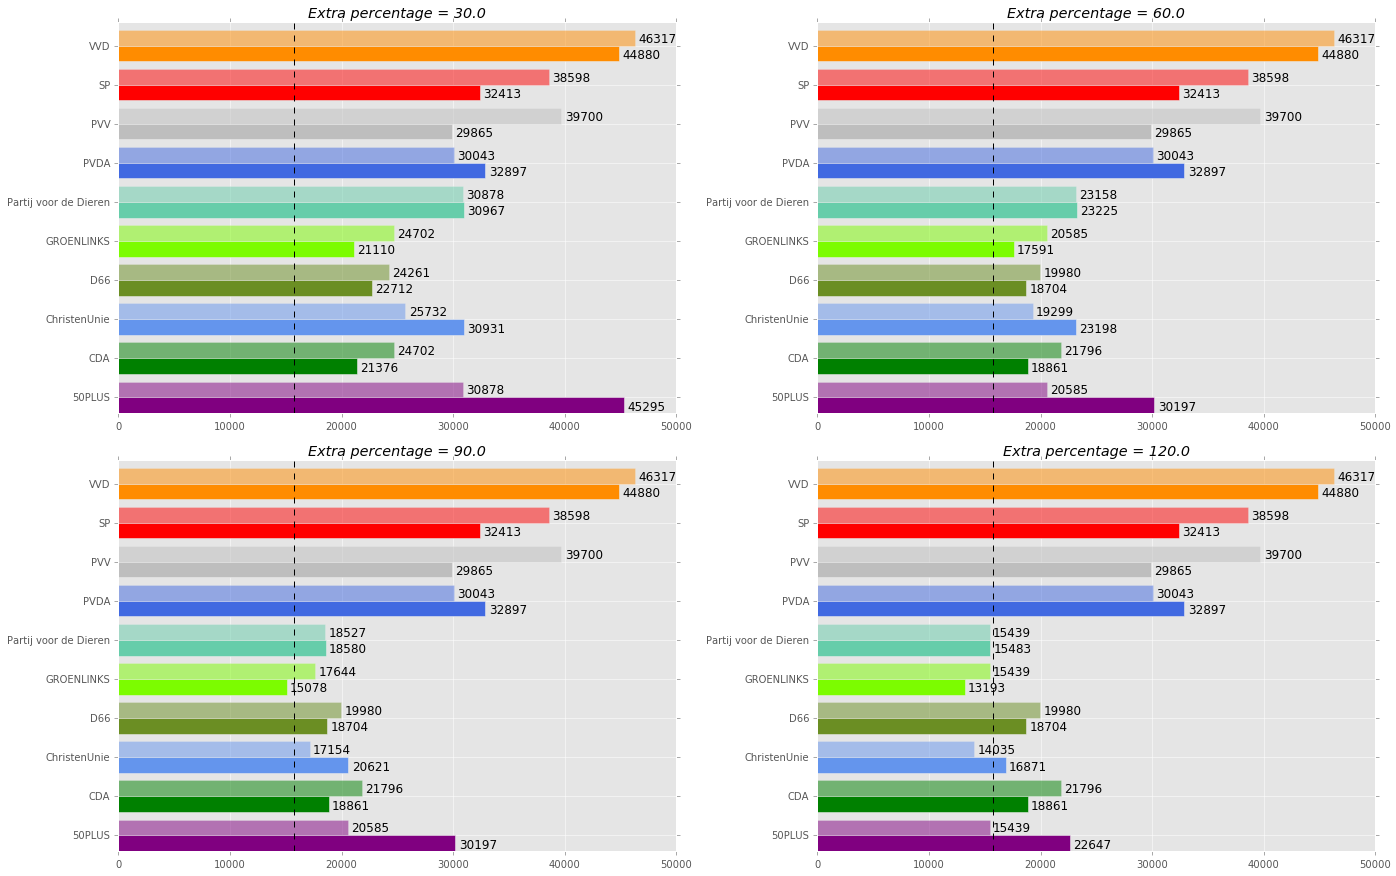
\includegraphics[width=\linewidth]	{stemmen_op_vrouwen_topNextrapercentage_samen.png}

			\caption{Grafieken in stappen van 30\%, met per partij de verdeling van de stemmen van vrouwelijke kiezers op de top \textit{N+extra percentage} vrouwelijke kandidaten van de partij a.d.h.v. de peiling (licht gekleurd) en a.d.h.v. de einduitslag (donker gekleurd). De stippellijn is de daadwerkelijk voorkeursdrempel(15.708 stemmen).}

\label{fig:stemmenS4V}
\end{figure}

In Figuur \ref{fig:stemmenS4V} hierboven, is te zien dat zowel volgens de peiling (voorspelling) alsmede volgens de einduitslag niet alle top \textit{N+extra percentage} vrouwelijke kandidaten van de partijen boven de daadwerkelijke voorkeursdrempel uitgekomen wanneer het \textit{extra percentage} aan zetels (voor vrouwelijke kandidaten) wordt verhoogd. Echter gebeurt dit pas tussen de 60\%  en 90\% extra zetels (voor vrouwelijke kandidaten) waarover de stemmen verdeeld worden. Ofschoon de precieze aantallen niet exact hetzelfde zijn, is met strategie 4 de voorspelling zoals berekend a.d.h.v. de peiling grotendeels correct in het voorspellen welke partijen met de top \textit{N+extra percentage} vrouwelijke kandidaten boven de voorkeursdrempel uitkomen en van welke partijen dit niet het geval is. Echter wordt voor sommige partijen verwacht dat de top \textit{N+extra percentage} vrouwelijke kandidaten boven de voorkeursdrempel uit zouden komen terwijl dit bij de einduitslag niet het geval blijkt te zijn en vice versa. Dit ligt ten grondslag aan het feit dat de er verschillen optreden in het aantal te verwachten stemmen op een partij (en het aantal te verwachten stemmen van vrouwelijke kiezers op een partij) volgens de peiling en het aantal ontvangen stemmen op een partij (en het aantal ontvangen stemmen van vrouwelijke kiezers op een partij) volgens de einduitslag.



\paragraph{Aantal vrouwen na strategie 4.}
Na het uitvoeren van strategie 4 en het opstellen van de Tweede Kamer zoals eerder in dit hoofdstuk beschreven, levert strategie 4 bij geen enkel \textit{extra percentage} bovenop de originele \textit{N} uit strategie 1 een hoger aantal vrouwen op in de Tweede Kamer. In de grafiek in Figuur \ref{fig:bcS4V} hieronder is te zien hoeveel vrouwen er in de Tweede Kamer een zetels bedeeld krijgen wanneer er een bepaald \textit{extra percentage} wordt toegevoegd aan de originele \textit{N} uit strategie 1.



\begin{figure}[H]

	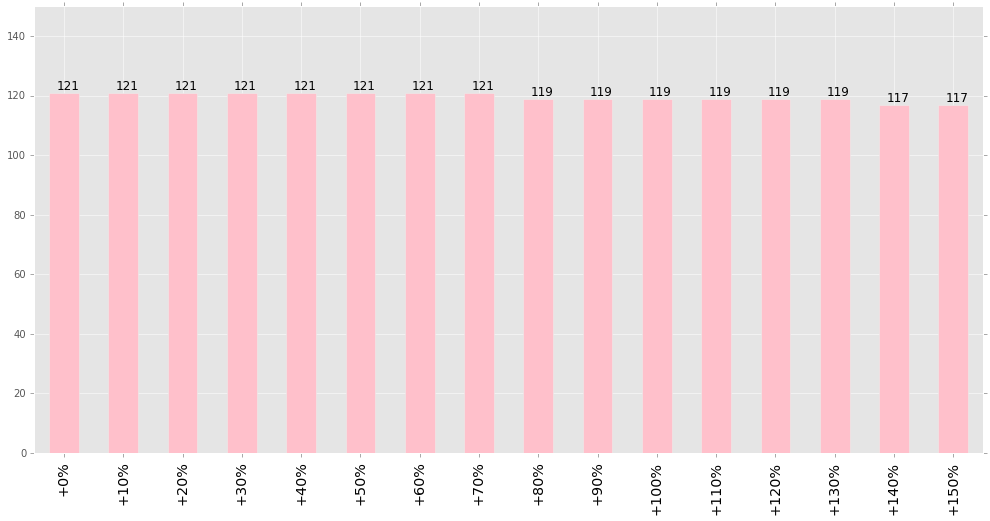
\includegraphics[width=\linewidth]	{topNextrapercentage_aantal_vrouwen_overzicht.png}

			\caption{Grafiek met per het aantal vrouwen in de Tweede Kamer na uitvoering(en) van strategie 4 in stappen van 10\% aan \textit{extra percentage} (van \textit{N}) bovenop de \textit{N} uit strategie 1.}

\label{fig:bcS4V}
\end{figure}

\paragraph{Niet meer maar minder vrouwen na uitvoering van strategie 4.}
Zoals hierboven in Figuur \ref{fig:bcS4V} te zien, komen er na uitvoering van strategie 4 en het toenemen van het \textit{extra percentage} op geen enkel moment meer vrouwen in de Tweede Kamer dan de 121 uit strategie 1 (0\% staat in de grafiek gelijk aan strategie 1.) 


\paragraph{Niet meer dan 121 vrouwen in de Tweede Kamer.}
De reden dat er niet meer dan 121 vrouwen in de Tweede Kamer plaatsnemen na uitvoering van strategie 4 ligt ten grondslag aan een aantal factoren. Willen er meer vrouwen in de Tweede Kamer plaatsnemen dan na uitvoering van strategie 1 dan is het noodzakelijk dat de partijen ook meer zetels kregen bedeeld bij de einduitslag dan dat volgens te peiling was te verwachten. 
\\
\indent Zo kreeg het CDA bij de einduitslag dertien zetels bedeeld terwijl de peilingen aangaf dat het CDA twaalf zetels kon gaan verwachten. Vanwege het feit dat zowel de lijsttrekker, in de persoon van Sybrand van Haersma Buma, alsmede Pieter Omtzigt meer stemmen ontvingen dan de vrouwelijke kandidaten, blijven er nog elf zetels over die aan vrouwelijke kandidaten bedeeld kunnen worden. Bij strategie 1 werden de zetels al bedeeld aan deze elf vrouwelijke kandidaten.
D66 kreeg bij de einduitslag twaalf zetels bedeeld terwijl de peiling aangaf dat D66 elf zetels kon gaan verwachten. Vanwege het feit dat de lijsttrekker, in de persoon van Alexander Pechtold, meer stemmen ontving dan de vrouwelijke kandidaten, blijven er nog elf zetels over die aan vrouwelijke kandidaten bedeeld kunnen worden. Bij strategie 1 werden er al elf zetels bedeeld aan vrouwelijke kandidaten. De PVDA kreeg bij de einduitslag 38 zetels bedeeld terwijl de peiling aangaf dat de PVDA 36 zetels kon gaan verwachten. Vanwege het feit dat zowel de lijsttrekker, in de persoon van Diederik Samsom, als Ronald Plasterk meer stemmen ontvingen dan de vrouwelijke kandidaten, blijven er nog 36 zetels over die aan de vrouwelijke kandidaten bedeeld kunnen worden. Bij strategie 1 werden er al 36 zetels bedeeld aan vrouwelijke kandidaten. Ook de VVD kreeg bij de einduitslag meer zetels bedeeld dan dat zij volgens de peiling konden gaan verwachten (36 zetels bij de peiling en 41 zetels bij de einduitslag). Echter had de VVD maar 24 vrouwelijke kandidaten op de lijst staan. Hierdoor werd de \textit{N+extra percentage} nooit meer dan 24 vrouwelijke kandidaten. Alle vrouwelijke stemmen op de VVD werden bij strategie 1 al verdeeld over alle 24 vrouwelijke kandidaten. 
\\
\indent De andere partijen ontvingen niet meer zetels bij de einduitslag dan dat zij volgens de peiling konden gaan verwachten. Zodoende kan het aantal vrouwen die in de Tweede Kamer plaatsnemen nooit op meer dan 121 uitkomen.   





